\documentclass[11pt]{article}
\usepackage[T1]{fontenc}
\usepackage[margin=1in]{geometry}
\usepackage{amsmath,amssymb}
\usepackage{graphicx}
\usepackage{booktabs}
\usepackage{xcolor}
\usepackage[colorlinks=true,linkcolor=blue!60!black,urlcolor=blue!60!black]{hyperref}
\usepackage{listings}
\lstset{basicstyle=\ttfamily\small, backgroundcolor=\color{gray!8},
        frame=single, rulecolor=\color{gray!40}, breaklines=true,
        columns=fullflexible, keepspaces=true}

\newcommand{\code}[1]{\texttt{#1}}
\newcommand{\kperp}{k_\perp}

\title{FFT Self-Gravity in the AthenaK Shearing Box:\\
       Implementation and Validation}
\author{\code{athenak-multigrid} tree, branch \code{multigrid}}
\date{August 3, 2026}

\begin{document}
\maketitle

\begin{abstract}
\noindent
This document records the design, mathematics, implementation, and validation of an
FFT-based self-gravity solver for AthenaK's shearing box, added to the
\code{athenak-multigrid} tree. The solver follows the Athena-C implementation in
\code{selfg\_fft\_disk.c}: the shearing-box phase-shift method of Gammie (2001) and the
open (vacuum) vertical boundary condition of Koyama \& Ostriker (2009), built on the
\code{kokkos-fft} library so the same code runs on CPU and GPU backends. Validation:
the triply periodic solve satisfies the discrete Poisson equation to machine precision
($3.8\times10^{-14}$); the shearing solve is exact at shear-periodic instants and
converges at the remap interpolation order (3rd for \code{ppmx}) against analytic
shearing-wave solutions; the open-boundary solve is exact in the interior and matches
the analytic slab potential to $0.15\%$; a Jeans-wave evolution agrees with the
existing multigrid solver to nine significant digits while running $3.5\times$ faster;
and a self-gravitating shearing wave reproduces linear swing-amplification theory
through the swing (peak amplification $3.62$ vs.\ $3.605$ predicted at $256^2$),
with the wave's phase locking to the instantaneous shearing wavevector holding to
$10^{-13}$ and the remaining $L_2$ difference shown to be hydrodynamic in origin
--- it is the same size in a control run with gravity switched off.
\end{abstract}

\tableofcontents

%=======================================================================
\section{Plan and scope}

\subsection{Goal and roadmap}
The scientific target is shearing-box simulations combining gas self-gravity, dust with
mutual drag (streaming instability, including the background radial pressure gradient),
and mesh refinement that zooms onto high dust-density regions in spiral arms launched by
gravitational instability (cf.\ Baehr, Zhu \& Yang 2022, ApJ 933, 100, who omitted the
pressure gradient). Because refinement is essential, the adopted route makes the
\emph{multigrid} solver shear-aware, with the FFT solver of this document retained in
three roles: the machine-precision \emph{oracle} for validating multigrid's shear BCs,
the production solver for uniform-grid runs, and the donor of exact open-$z$ Dirichlet
boundary values for stratified multigrid runs. The phases:
\begin{enumerate}
  \item \textbf{(done; Secs.~2--5)} Uniform-grid FFT Poisson solver: shearing-periodic
        horizontal boundaries (Gammie 2001 phase shift), periodic or open vertical
        boundaries (Koyama \& Ostriker 2009), validated through swing amplification.
  \item \textbf{(done)} Phase 0: shearing box + mesh refinement infrastructure ---
        interior-$x_1$ refinement policy, a non-FARGO mode, and orbital advection
        (FARGO) on refined meshes under an annular refinement policy. Documented
        separately in \code{multigrid\_selfgravity\_validation.pdf}, which covers the
        multigrid/refinement track.
  \item Phase 1--2: shear-periodic boundary conditions in the multigrid driver,
        validated against the FFT solver of this document as a machine-precision
        oracle; then multigrid gravity on refined shearing-box meshes.
  \item Phase 3--5: merge with the \code{athenak-dust} particle-mesh dust module
        (dust density in the Poisson source, gravity on particles, pressure-gradient
        source term), stratification with open-$z$ boundaries, and science runs.
\end{enumerate}

\subsection{Version-1 scope}
The solver currently \emph{requires} (and enforces with fatal errors): a 3D mesh, a
uniform grid (no SMR/AMR --- AthenaK already forbids refinement with a shearing box),
a single MPI rank, and (shear-)periodic $x_1$/$x_2$ boundaries. The vertical boundary
is periodic (with mean-density subtraction) or open. Shearing and non-shearing cases
share one code path: with shear rate $q=0$ every shear-specific step reduces to the
identity.

%=======================================================================
\section{Numerical method}

\subsection{The discrete Poisson equation and its exact k-space inverse}
The gravity source terms difference the potential with second-order central
differences, so the solver targets the \emph{finite-difference} Poisson equation
\begin{equation}
  (L\Phi)_{ijk} \;\equiv\;
  \frac{\Phi_{i+1}-2\Phi_i+\Phi_{i-1}}{\Delta x^2} +
  \frac{\Phi_{j+1}-2\Phi_j+\Phi_{j-1}}{\Delta y^2} +
  \frac{\Phi_{k+1}-2\Phi_k+\Phi_{k-1}}{\Delta z^2}
  \;=\; 4\pi G\,\rho_{ijk},
  \label{eq:discrete}
\end{equation}
not the continuum equation. On a periodic uniform grid the DFT modes
$e^{\mathrm{i}k_x x_i}$ are eigenvectors of each difference operator: applying the
stencil to $e^{\mathrm{i}k_x i\Delta x}$ and factoring out the mode gives the
eigenvalue
\begin{equation}
  D(\mathbf{k}) = \frac{2\cos(k_x\Delta x)-2}{\Delta x^2}
                + \frac{2\cos(k_y\Delta y)-2}{\Delta y^2}
                + \frac{2\cos(k_z\Delta z)-2}{\Delta z^2}
  \;\xrightarrow{\;k\Delta\to0\;}\; -k^2 .
  \label{eq:Dk}
\end{equation}
The solve is therefore: FFT $4\pi G\rho$, divide each mode by $D(\mathbf{k})$,
inverse FFT. Because $D$ is the exact symbol of the same stencil later used to
compute forces, the returned $\Phi$ satisfies Eq.~\eqref{eq:discrete} to machine
precision --- there is no iteration residual (contrast multigrid). The
$\mathbf{k}=0$ mode is set to zero, which is exactly equivalent to subtracting the
mean density (the Jeans swindle, required for consistency of the periodic problem).

\subsection{Shearing box: the phase-shift (rolled-frame) method}
\label{sec:shear}
With background velocity $v_{y,0}=-q\Omega x$, the shearing-periodic boundary
condition identifies
\begin{equation}
  \rho(x,\,y,\,z,\,t) \;=\; \rho(x+L_x,\; y - q\Omega L_x t,\; z,\; t),
\end{equation}
so the box is strictly periodic only at times $t_n=n\,T_{\rm sh}$ with
$T_{\rm sh}=L_y/(q\Omega L_x)$. Let $t_s$ be the time since the most recent $t_n$
and $\theta \equiv q\Omega t_s$ (code variable \code{qomt}). In sheared coordinates
$y' = y + \theta x$ the density \emph{is} doubly periodic:
\begin{equation}
  \rho'(x,\,y',\,z) = \rho(x,\; y'-\theta x,\; z)
  \qquad\Longleftrightarrow\qquad
  \text{``roll'': shift each $x$-column of content by } +\theta x \text{ in } y .
  \label{eq:roll}
\end{equation}
A rolled-frame mode $e^{\mathrm{i}(k_x'x + k_y y')}$ is a shearing wave with
\emph{physical} radial wavenumber
\begin{equation}
  k_x = k_x' + \theta\,k_y
  \qquad\text{(index form: } k_x\Delta x = \bigl(i_p + \theta\,\tfrac{L_x}{L_y}\,j_p\bigr)\tfrac{2\pi}{N_x}\text{)},
  \label{eq:kxshift}
\end{equation}
with $j_p$ the \emph{signed} mode index. The pipeline is: roll $\rho$
$\to$ FFT $\to$ divide by $D(k_x'{+}\theta k_y,\,k_y,\,k_z)$ $\to$ inverse FFT
$\to$ unroll $\Phi$ (shift by $-\theta x$).

A point worth recording: if the roll/unroll used \emph{spectral} (Fourier)
interpolation, the composite operation would invert Eq.~\eqref{eq:discrete}
exactly at all times --- the per-column shift is then a pure phase factor
$e^{\mathrm{i}k_y\theta x}$, under which the unsheared stencil pulls back exactly
to the shifted-eigenvalue form of Eq.~\eqref{eq:kxshift}. All error at
$\theta\neq0$ therefore comes from the finite-order remap interpolation, and the
solver is exact whenever $\theta=0$ (verified below to $3\times10^{-14}$).

The remap is the conservative flux form shared with AthenaK's orbital
advection (\code{remap\_fluxes.hpp}): the integer part of the shift is folded
into a periodic-wrapped load, the fractional part $\epsilon\in(-1,1)$ is applied as
$q_j \to q_j - (F_{j+1}-F_j)$ with upwind flux kernels of first
(\code{dc}), second (\code{plm}), or third (\code{ppmx}) order. As a
\emph{static} remap, donor-cell reduces to linear interpolation (2nd-order
pointwise), \code{plm} is 2nd order with a smaller constant, and \code{ppmx} is 3rd
order --- exactly the orders measured in Sec.~\ref{sec:tests}.

\paragraph{Ghost zones.} The gravity source term needs one valid face-adjacent ghost
layer of $\Phi$. Interior meshblock faces come from the global solution; $x_2$
ghosts wrap periodically; the physical $x_1$ ghost planes use the shear-periodic
identification: the inner ghost plane is the outer boundary column with content
shifted by $+\theta L_x$ (mod $L_y$), and vice versa, using the same remap kernel.

\subsection{Open vertical boundary: the two-solve method (Koyama \& Ostriker 2009)}
\label{sec:openbc}
Fourier transforming horizontally, each mode obeys
$(\mathrm{d}^2/\mathrm{d}z^2 - \kperp^2)\hat\Phi = 4\pi G\hat\rho$, whose isolated
(vacuum) solution is the screened kernel
$\hat\Phi(z) = -\tfrac{2\pi G}{\kperp}\!\int\!\hat\rho(z')\,
e^{-\kperp|z-z'|}\mathrm{d}z'$.
A vertically periodic solve instead delivers an infinite stack of image slabs
separated by $L_z$:
\begin{equation}
  S_p = \sum_{n=-\infty}^{\infty} e^{-\kperp|z-z'-nL_z|}
      = \frac{e^{-\kperp\zeta}+e^{-\kperp(L_z-\zeta)}}{1-q},
  \qquad q\equiv e^{-\kperp L_z},\;\; \zeta = z-z' \in[0,L_z).
\end{equation}
A second solve on $4\pi G\rho\,e^{-\mathrm{i}\pi z/L_z}$ shifts the vertical
spectrum by half a wavenumber (half-integer harmonics $=$ \emph{antiperiodic}
vertical extension), whose Green's function is the alternating stack
\begin{equation}
  S_a = \sum_{n} (-1)^n e^{-\kperp|z-z'-nL_z|}
      = \frac{e^{-\kperp\zeta}-e^{-\kperp(L_z-\zeta)}}{1+q}.
\end{equation}
Both are combinations of the same two functions of $\zeta$; solving the
$2\times2$ system for the weights that cancel the wraparound term and normalize
the vacuum kernel gives
\begin{equation}
  \boxed{\;\alpha_p = \tfrac12\,(1 - e^{-\kperp L_z}), \qquad
         \alpha_a = \tfrac12\,(1 + e^{-\kperp L_z}),\qquad
         \alpha_p S_p + \alpha_a S_a = e^{-\kperp\zeta}. \;}
\end{equation}
Every periodic image cancels identically; the result is the isolated-slab
potential at the cost of one extra FFT pair. In k-space, solve A multiplies by
$\alpha_p/D(k_x',k_y,k_z^{\rm int})$ and solve B by
$\alpha_a/D(k_x',k_y,k_z^{\rm half})$ with $k_z^{\rm half}\Delta z =
(m+\tfrac12)\,2\pi/N_z$; the recombination is
$\Phi = \Phi_A + \mathrm{Re}\!\left[e^{+\mathrm{i}\pi \tilde z/L_z}\Phi_B\right]$
with cell-centered $\tilde z = z - z_{\min}$.

At $\kperp=0$ the weights become $(0,1)$: the horizontally averaged density is
carried entirely by the antiperiodic solve, which correctly reproduces the linear
$|z|$-type slab potential; no mean-density subtraction occurs in open mode, and the
$D=0$ singularity never arises. Matching Athena-C, the screening exponent uses the
\emph{continuum} $\kperp = [(k_x\Delta x/\Delta x)^2+(k_y\Delta y/\Delta y)^2]^{1/2}$
(with the shear-shifted $k_x$) rather than the discrete decay rate $\kappa$ defined
by $2[\cosh(\kappa\Delta z)-1]/\Delta z^2 = k_{\perp,\rm eff}^2$; the difference
matters only where $e^{-\kperp L_z}$ is already exponentially negligible. The $x_3$
ghost layer is filled by linear extrapolation in open mode (the layers touching it
are excluded from ``interior'' error norms).

\subsection{Cost and normalization}
Periodic mode: one complex-to-complex FFT pair per solve. Open mode: two pairs.
FFT plans are created once and reused; normalization is the NumPy convention
(inverse transform carries $1/N$), passed explicitly. Kernel coefficients
(Eqs.~\ref{eq:Dk},~\ref{eq:kxshift}) are computed on the fly inside the k-space
multiply --- they are time-dependent through $\theta$, and recomputing costs less
than storing. The solve runs once per Runge--Kutta stage, matching the multigrid
convention, so the potential is consistent with the stage's density.

%=======================================================================
\section{What was built}
\label{sec:impl}

\subsection{New and modified files}
\begin{center}
\small
\begin{tabular}{@{}ll@{}}
\toprule
File & Content \\
\midrule
\code{src/gravity/fft\_gravity.hpp} & \code{FFTGravitySolver} class declaration \\
\code{src/gravity/fft\_gravity.cpp} & solver implementation (all kernels) \\
\code{src/gravity/gravity.\{hpp,cpp\}} & solver switch, \code{Gravity::Solve()} dispatch \\
\code{src/driver/driver.cpp} & one line: \code{pgrav->Solve(this,stage)} \\
\code{src/multigrid/multigrid.hpp} & pre-existing fix: \code{Smooth} moved out-of-line$^\dagger$ \\
\code{src/pgen/tests/fft\_poisson.cpp} & validation problem generator (+ registration) \\
\code{src/pgen/tests/swing.cpp} & swing-amplification pgen + user history function \\
\code{CMakeLists.txt}, \code{src/CMakeLists.txt}, \code{config.hpp.in} & build integration \\
\code{inputs/tests/*.athinput} & test inputs (fft\_poisson*, jeans\_fft, swing) \\
\code{validation/} & this document, figures, Julia notebook \\
\bottomrule
\end{tabular}
\end{center}
\noindent {\footnotesize $^\dagger$ \code{Multigrid::Smooth} accessed the not-yet-defined
\code{MultigridDriver} inside the class body; Apple clang~21 rejects this, so the
template body was moved below the driver class definition. No behavior change; the
multigrid Jeans test still passes.}

\subsection{Solver pipeline}
\code{FFTGravitySolver::Solve()} executes, per RK stage:
\begin{enumerate}
  \item \textbf{Gather}: active-zone density from all meshblocks into a global
        $(N_z,N_y,N_x)$ device array (block offsets from logical locations),
        scaled by $4\pi G$.
  \item \textbf{Roll}: conservative per-column $y$-shift by $+\theta x$
        (Eq.~\ref{eq:roll}); identity when $\theta=0$.
  \item \textbf{k-space solve}: periodic (one FFT pair) or open (two pairs,
        Sec.~\ref{sec:openbc}), with the shear-shifted kernel
        (Eq.~\ref{eq:kxshift}).
  \item \textbf{Unroll}: shift by $-\theta x$.
  \item \textbf{Ghost planes}: shear-periodic $x_1$ ghost columns
        ($\pm\theta L_x$ shifts).
  \item \textbf{Scatter}: into \code{pgrav->phi} (active zones + one ghost layer);
        the unchanged \code{SelfGravity} source term consumes it.
\end{enumerate}
The multi-rank seam: steps 1 and 6 are the only places that assume the pack spans
the mesh; an \code{MPI\_Allgatherv} between local gather and roll (and a rank-local
scatter) upgrades the solver without touching steps 2--5.

\subsection{Runtime options}
\begin{center}
\begin{tabular}{@{}llll@{}}
\toprule
Block/parameter & Values & Default & Meaning \\
\midrule
\code{<gravity> solver} & \code{multigrid} $|$ \code{fft} & \code{multigrid} & Poisson solver selection \\
\code{<gravity> four\_pi\_G} & real & $-1$ (unset) & $4\pi G$ (pgens may override) \\
\code{<gravity> vert\_bc} & \code{periodic} $|$ \code{open} & \code{periodic} & vertical boundary \\
\code{<gravity> fft\_remap} & \code{dc} $|$ \code{plm} $|$ \code{ppmx} & \code{plm} & $y$-remap order \\
\code{<shearing\_box> qshear, omega0} & real & --- & read if the block exists \\
\code{<hydro\_srcterms> self\_gravity} & bool & false & enable source term \\
\bottomrule
\end{tabular}
\end{center}
Existing multigrid input files run unchanged (default \code{solver=multigrid}).

%=======================================================================
\section{Building and compiling}

Prerequisites (done once; already satisfied on this machine):
\begin{lstlisting}
cd athenak-multigrid
git submodule update --init kokkos     # Kokkos 4.7.02, vendored
brew install fftw                      # host FFT backend for kokkos-fft
\end{lstlisting}
Configure and build (kokkos-fft v2.0.0 is fetched automatically by CMake;
it consumes the in-tree Kokkos target and links FFTW on host backends,
cuFFT/hipFFT on GPU backends):
\begin{lstlisting}
mkdir build && cd build
cmake -D Athena_ENABLE_FFT=ON ..
make -j8
\end{lstlisting}
Without \code{-D Athena\_ENABLE\_FFT=ON} the code builds exactly as before;
requesting \code{solver=fft} then aborts with an explanatory error.

%=======================================================================
\section{Tests and results}
\label{sec:tests}

All tests use the \code{fft\_poisson} problem generator, which fills a
deterministic density field, calls the gravity solve once, and prints error
diagnostics (lines starting \code{\# FFT-POISSON}). Initial conditions are
selected by \code{<problem> profile = modes | shwave | slab} and are overridable
on the command line. The companion Julia notebook
(\code{validation/fft\_selfgravity\_tests.ipynb}) re-runs every test and checks
the outputs independently of the C++ diagnostics.

\subsection{Discrete consistency (periodic, no shear)}
Multi-mode + Gaussian-blob density, $64^3$, 8 meshblocks:
\begin{lstlisting}
./build/src/athena -i inputs/tests/fft_poisson.athinput
# FFT-POISSON ERRORS: max_rel_all= 3.757e-14  l2_rel_all= 1.216e-14
\end{lstlisting}
The 7-point Laplacian of the returned potential reproduces
$4\pi G(\rho-\bar\rho)$ at machine precision, confirming the k-space inversion,
the multi-block gather/scatter, and the periodic ghost fill simultaneously.

\subsection{Shear bookkeeping: exactness at shear-periodic instants}
Same field in a $q=1.5$, $\Omega=1$ shearing box ($T_{\rm sh}=2/3$):
solving at $t=T_{\rm sh}$ (i.e.\ $\theta=0$) returns
\code{max\_rel = 3.0e-14} --- the entire shear code path (roll, shifted kernel,
unroll, shear ghosts) collapses to the exact periodic solve, as it must.
At a generic phase ($t_0=0.37$, $\theta=0.555$) the residual is finite and
dominated by remap interpolation, as designed; see the caveat below.
Figure~\ref{fig:phase} sweeps the shear phase across a full period: the residual
drops by twelve orders of magnitude precisely at $t_0=0$ and $t_0=T_{\rm sh}$ and
is flat in between, confirming that the modular shear-phase arithmetic
($\theta = q\Omega\,[t \bmod T_{\rm sh}]$) has exactly the right period and that
no error accumulates with time.

\begin{figure}[htb]
  \centering
  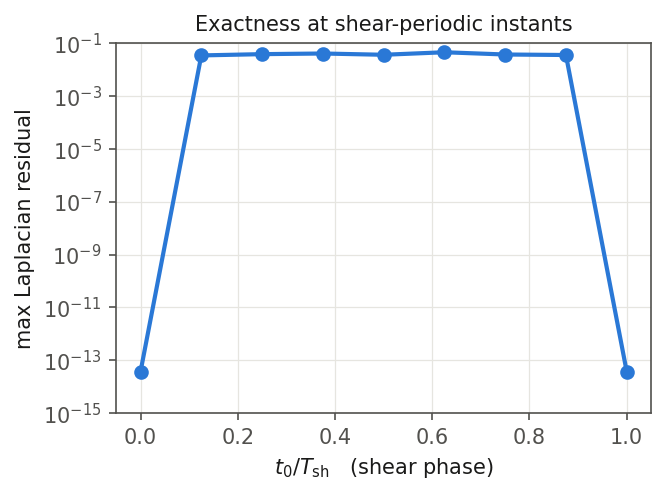
\includegraphics[width=0.58\textwidth]{figures/phase_sweep.png}
  \caption{Laplacian residual versus shear phase over one shear period
  ($64^3$, \code{modes} profile, \code{ppmx} remap). The solve is exact to
  machine precision exactly when the box is strictly periodic.}
  \label{fig:phase}
\end{figure}

\subsection{Shearing-wave solutions: order-of-accuracy}
For a single rolled-frame mode $(n_1,n_2,n_3)$ the exact discrete solution is
known analytically: the same slanted wave with amplitude
$4\pi G\,\delta\rho/D$, $D$ evaluated with the shifted $k_x$
(Eq.~\ref{eq:kxshift}). Figure~\ref{fig:conv} shows the pointwise potential
error at $\theta=0.555$. Measured orders per resolution doubling:
\code{ppmx} $3.08,\,3.02$; \code{plm} $2.02,\,2.01$; \code{dc} $1.94,\,2.05$ ---
precisely the remap interpolation orders. Figure~\ref{fig:slice} shows the slanted wave and the
solved potential (correlation coefficient $-1.0$ to $10^{-11}$: potential wells
align with density crests).

\begin{figure}[htb]
  \centering
  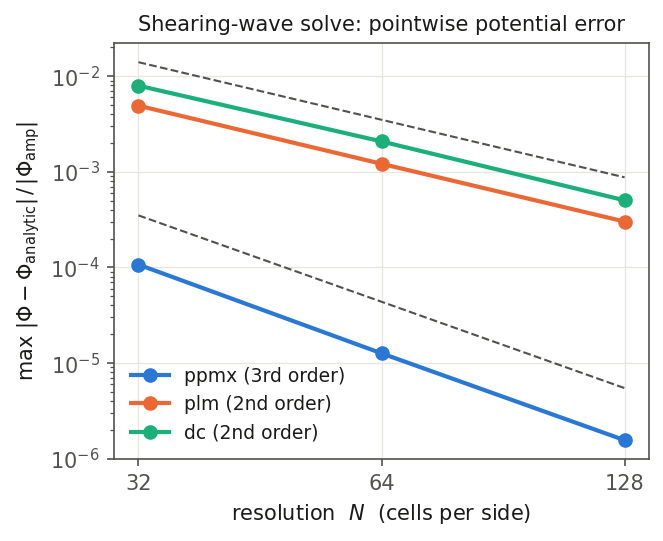
\includegraphics[width=0.62\textwidth]{figures/convergence.png}
  \caption{Maximum pointwise error of $\Phi$ against the analytic discrete
  shearing-wave solution, mode $(1,1,1)$, $q\Omega t_s = 0.555$, versus
  resolution, for the three remap orders. Dashed guides: $N^{-2}$, $N^{-3}$.}
  \label{fig:conv}
\end{figure}

\begin{figure}[htb]
  \centering
  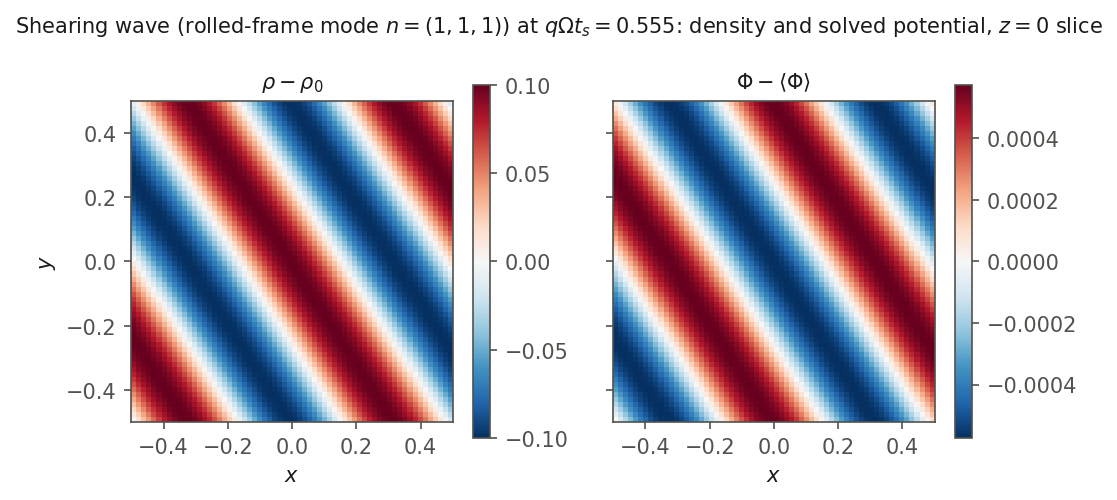
\includegraphics[width=0.95\textwidth]{figures/shwave_slice.png}
  \caption{$z=0$ slice of the shearing-wave test at $64^3$: density perturbation
  (left) and solved potential (right). The wavefronts are slanted by the
  accumulated shear; $\Phi$ is exactly anticorrelated with $\delta\rho$.}
  \label{fig:slice}
\end{figure}

\paragraph{A caveat on metrics (important when re-validating).}
Under shear, the \emph{Laplacian residual} of the returned potential is
\emph{not} a clean convergence metric: differencing divides the
$O(\Delta y^{\,p})$ remap interpolation error by $\Delta^2$, so the residual
improves only at roughly first order (and the max-norm can stall at
under-resolved sharp features, where the \code{ppmx} limiter locally reduces
order). This is intrinsic to the method --- with spectral interpolation the
residual would be exactly zero --- and is why the pointwise-$\Phi$ comparison of
Fig.~\ref{fig:conv} is the correct order-of-accuracy test. The printed
\code{max\_rel\_int}/\code{l2\_rel\_int} norms exclude boundary layers whose
ghosts are themselves interpolated (shear $x_1$ layers, extrapolated open-BC
$x_3$ layers).

\subsection{Open vertical boundary: slab potential}
A horizontally uniform $\rho = \rho_0\,\mathrm{sech}^2(z/H)$ slab with $H=L_z/20$
at $64^3$, \code{vert\_bc=open}:
interior residual \code{4.2e-14} (machine precision --- for this profile only the
$\kperp=0$ column is active, where the two-solve weights are exact), and the
$\Phi(z)$ profile matches the analytic infinite-slab potential
$4\pi G\rho_0 H^2 \ln\cosh(z/H)$ to $0.15\%$ (Fig.~\ref{fig:slab}); the residual
peaks at the slab center (finite-difference discretization of the sharp maximum)
and is limited by the truncated sech$^2$ wings at the box scale.

\begin{figure}[htb]
  \centering
  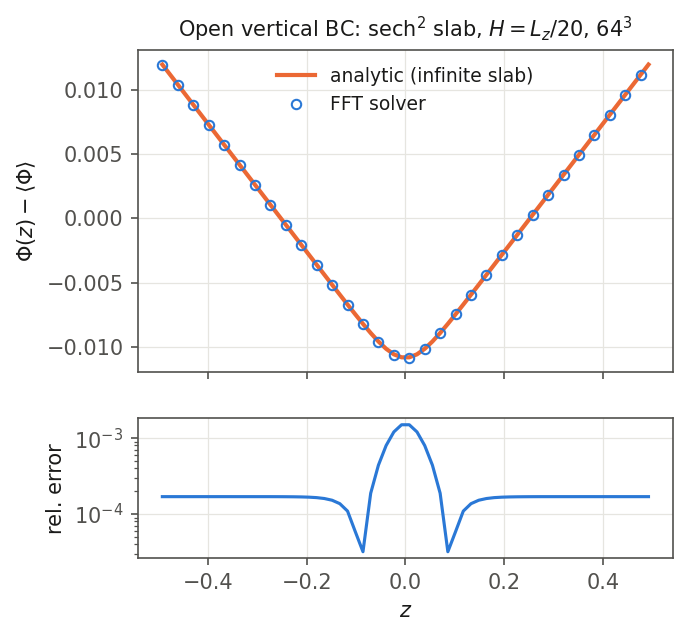
\includegraphics[width=0.6\textwidth]{figures/slab_profile.png}
  \caption{Open-BC slab test: solved $\Phi(z)$ (circles) versus the analytic
  infinite-slab potential (line), both zero-mean; lower panel: pointwise
  relative error.}
  \label{fig:slab}
\end{figure}

\subsection{End-to-end evolution: Jeans wave, FFT vs.\ multigrid}
The existing Jeans-wave test (\code{pgen\_name=gravity}) evolved to $t=1$
(321 cycles, RK2 $\Rightarrow$ 642 Poisson solves, 128 meshblocks of $8^3$):
\begin{center}
\begin{tabular}{@{}lccc@{}}
\toprule
 & mode amplitude at $t{=}1$ & wall time & zone-cycles/s \\
\midrule
FFT (\code{jeans\_fft.athinput}) & $-7.395719378\times10^{-7}$ & 6.6 s & $3.2\times10^6$ \\
Multigrid (\code{jeans\_wave.athinput}) & $-7.395719385\times10^{-7}$ & 22.9 s & $0.9\times10^6$ \\
\bottomrule
\end{tabular}
\end{center}
Agreement to nine significant digits (the difference is the multigrid iteration
residual; the FFT solve is exact), with a $3.5\times$ end-to-end speedup on this
serial-CPU build. This exercises the full loop: per-stage solve, source-term
coupling, and boundary/ghost handling during evolution.

\subsection{Swing amplification: gravity coupled to the dynamics}
\label{sec:swing}
All tests above check the Poisson solve in isolation. This one closes the loop:
solver $\to$ source term $\to$ hydrodynamics, in a shearing frame.

A leading shearing wave ($k_{x0}<0$, $k_y>0$, $k_z=0$) of small amplitude
($A=10^{-4}$) is wound up by the background shear, $k_x(t)=k_{x0}+q\Omega k_y t$;
as it swings through $k_x=0$ self-gravity transiently amplifies it (Goldreich \&
Lynden-Bell 1965; Julian \& Toomre 1966; Toomre 1981). Linearizing the isothermal
shearing-box equations for one shearing wave, with
$\delta=\delta\rho/\rho_0$ and $w_{x,y}=i\hat v_{x,y}$ (so
$v = w\sin\mathbf{k}\!\cdot\!\mathbf{x}$ while $\delta\propto\cos$):
\begin{equation}
  \delta' = -(k_x w_x + k_y w_y),\quad
  w_x' = 2\Omega w_y + k_x S,\quad
  w_y' = -(2-q)\Omega w_x + k_y S,\quad
  S = \delta\Bigl(c_s^2 + \frac{4\pi G\rho_0}{D}\Bigr),
  \label{eq:swingode}
\end{equation}
where $D$ is the solver's own discrete eigenvalue (Eq.~\ref{eq:Dk}, $\to-k^2$ in the
continuum). Eq.~\eqref{eq:swingode} is derived from the shearing-box equations in
Appendix~\ref{app:swing}; setting $k_y=0$ there recovers the Jeans dispersion relation
$\delta''=-(k^2c_s^2-4\pi G\rho_0)\delta$, one of three checks collected
in~\ref{app:checks}.

Parameters are chosen in the epicyclic-resonant regime where swing is strong:
$L_x=L_y=2\pi$, $n_{wy}=1$ so $k_y=1=\kappa$ (with $\kappa^2=2(2-q)\Omega^2=1$ at
$q=1.5$), and $4\pi G\rho_0 = 1.9$, just below the marginal value
$k_y^2c_s^2+\kappa^2=2$ --- so the swinging wave is strongly amplified while every
box mode remains Jeans-stable. Starting from $n_{wx}=-6$ the swing occurs at
$t_{\rm swing} = -n_{wx}/(q\,n_{wy}) = 4$, and the run covers $t\in[0,8]$
(12 shear periods). The \code{swing} problem generator projects the solution onto
the \emph{instantaneous} wavevector each history dump, giving $\delta$, $w_x$, $w_y$
directly.

\begin{figure}[htb]
  \centering
  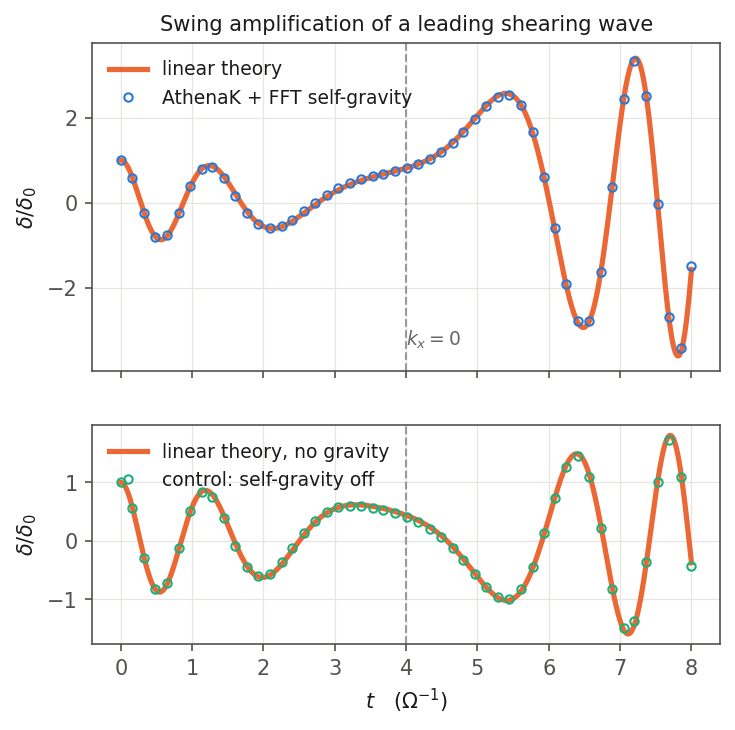
\includegraphics[width=0.62\textwidth]{figures/swing.png}
  \caption{Swing amplification at $128^2\times16$. Top: density amplitude of the
  shearing wave versus time, simulation (circles) against the linear ODE
  (Eq.~\ref{eq:swingode}, line); dashed line marks $k_x=0$. Bottom: the same run
  with self-gravity disabled, against the $4\pi G = 0$ theory --- no amplification.}
  \label{fig:swing}
\end{figure}

Results (Fig.~\ref{fig:swing}): the simulation tracks the linear solution through
the entire swing, reaching a peak amplification of $3.51$ against the predicted
$3.60$, with relative $L_2$ differences of $9\times10^{-3}$ ($\delta$),
$8\times10^{-3}$ ($w_x$) and $1.3\times10^{-2}$ ($w_y$) over the whole run at
$128^2$. Two sharper diagnostics:
\begin{itemize}
  \item The $k_x=0$ crossing recorded in the history file occurs at $t=4.005$
        against the predicted $4.000$ --- the shear-phase bookkeeping is right
        after twelve shear periods.
  \item The \emph{sine} projection of the density stays at
        $|\delta_{\sin}|/|\delta|_{\max} \sim 10^{-13}$ throughout. Linear theory
        says the wave stays exactly in phase with $\cos(\mathbf{k}(t)\!\cdot\!\mathbf{x})$;
        the simulation reproduces that phase locking to machine precision, which is
        a far more stringent statement than the amplitude agreement.
\end{itemize}
The residual $\sim$1\% difference is hydrodynamic truncation error, not a gravity
error. Table~\ref{tab:swingconv} makes that quantitative by repeating the
resolution study with self-gravity disabled, comparing each run against its own
linear theory ($4\pi G = 1.9$ and $4\pi G = 0$ respectively). Two things follow:
\begin{itemize}
  \item The peak amplification converges cleanly onto the predicted value,
        $2.64 \to 3.51 \to 3.62$ against $3.605$ (a $0.4\%$ difference at
        $256^2$), while the control converges onto its own, much smaller,
        gravity-free value ($1.80$ vs.\ $1.49$ predicted --- the control is
        \emph{not} amplified).
  \item At $256^2$ the two $L_2$ errors are equal to within 3\%
        ($4.10\times10^{-3}$ with gravity, $3.99\times10^{-3}$ without).
        An error that is the same size whether or not the Poisson solver is
        running cannot originate in the Poisson solver: it is the
        PLM/HLLE/RK2 discretization of the hydrodynamics, which the linear ODE
        does not model. (The gravity-on sequence is non-monotonic in apparent
        order only because its $64^2$ point is badly under-resolved --- the peak
        amplitude is off by 27\% there.)
\end{itemize}

\begin{table}[htb]
  \centering
  \caption{Swing solution versus linear theory (relative $L_2$ over $t\in[0,8]$,
  each run compared against theory with its own $4\pi G$).}
  \label{tab:swingconv}
  \begin{tabular}{@{}lcccc@{}}
  \toprule
   & \multicolumn{2}{c}{self-gravity ON} & \multicolumn{2}{c}{self-gravity OFF (control)} \\
  \cmidrule(lr){2-3}\cmidrule(lr){4-5}
  resolution & peak $\delta/\delta_0$ & $L_2$ error & peak $\delta/\delta_0$ & $L_2$ error \\
  \midrule
  $64^2\times16$  & 2.638 & $9.08\times10^{-2}$ & 1.275 & $9.78\times10^{-2}$ \\
  $128^2\times16$ & 3.511 & $8.97\times10^{-3}$ & 1.734 & $1.81\times10^{-2}$ \\
  $256^2\times16$ & 3.619 & $4.10\times10^{-3}$ & 1.801 & $3.99\times10^{-3}$ \\
  \midrule
  linear theory   & 3.605 & --- & 1.490 & --- \\
  \bottomrule
  \end{tabular}
\end{table}

\subsection{Reproducing}
\begin{lstlisting}
# periodic consistency
./build/src/athena -i inputs/tests/fft_poisson.athinput
# shear: generic phase / periodic instant
./build/src/athena -i inputs/tests/fft_poisson_shear.athinput
./build/src/athena -i inputs/tests/fft_poisson_shear.athinput \
                   problem/time0=0.6666666666666667
# shearing-wave convergence (vary N, gravity/fft_remap, problem/n1..n3)
./build/src/athena -i inputs/tests/fft_poisson_shear.athinput \
    problem/profile=shwave gravity/fft_remap=ppmx \
    mesh/nx1=64 mesh/nx2=64 mesh/nx3=64 \
    meshblock/nx1=64 meshblock/nx2=64 meshblock/nx3=64
# open-BC slab
./build/src/athena -i inputs/tests/fft_poisson_open.athinput
# Jeans evolution
./build/src/athena -i inputs/tests/jeans_fft.athinput
# swing amplification (writes SwingSG.user.hst); control run without gravity:
./build/src/athena -i inputs/tests/swing_selfgrav.athinput
./build/src/athena -i inputs/tests/swing_selfgrav.athinput \
    job/basename=SwingNoG128 hydro_srcterms/self_gravity=false
\end{lstlisting}
Each run writes \code{bin/*.bin} snapshots (\code{hydro\_w}, \code{grav\_phi})
that the Julia notebook reads. Figures in this document are regenerated by
\code{validation/figures/make\_figures.py}.

%=======================================================================
\section{Next steps}
\begin{enumerate}
  \item Multi-rank support (\code{MPI\_Allgatherv} at the seam documented in
        Sec.~\ref{sec:impl}), lifting the single-rank restriction.
  \item Python regression harness under \code{tst/test\_suite/fft\_gravity/}
        mirroring the multigrid suite, so these checks run in CI.
  \item The FFT-root + multigrid-refinement hybrid for the AMR goal: the FFT solve
        on the uniform root grid supplies both the global solution and, by
        prolongation, Dirichlet boundary data for multigrid on refined interior
        patches --- which never touch the shear-periodic boundary.
  \item Physics extensions once the above land: star-particle deposition into the
        density field (skipped in the Athena-C shearing branch, see
        Sec.~\ref{sec:impl}), and stratified shearing boxes combining
        \code{vert\_bc=open} with vertical gravity.
\end{enumerate}

%=======================================================================
\appendix
\section{\texorpdfstring{Derivation of the linearized shearing-wave system,
         Eq.~\eqref{eq:swingode}}{Derivation of the linearized shearing-wave system}}
\label{app:swing}

This appendix derives Eq.~\eqref{eq:swingode} --- the reference solution against which
the swing test of Sec.~\ref{sec:swing} is compared --- from the shearing-box equations.
Three checkpoints for verifying the algebra are collected in \ref{app:checks}.

\subsection{Shearing-box equations and the background state}
The shearing box is a local Cartesian frame co-rotating at radius $R_0$ with angular
velocity $\mathbf{\Omega}=\Omega\hat z$; coordinates $(x,y,z)$ are (radial, azimuthal,
vertical) with $x = R-R_0$. For an isothermal, unstratified gas ($P=c_s^2\rho$, no
vertical external gravity):
\begin{equation}
  \frac{\partial\rho}{\partial t} + \nabla\cdot(\rho\mathbf{v}) = 0,
  \qquad
  \frac{\partial\mathbf{v}}{\partial t} + (\mathbf{v}\cdot\nabla)\mathbf{v}
  = -\frac{c_s^2}{\rho}\nabla\rho - \nabla\Phi
    \underbrace{-\,2\mathbf{\Omega}\times\mathbf{v}}_{\text{Coriolis}}
    + \underbrace{2q\Omega^2 x\,\hat x}_{\text{tidal}},
  \label{eq:sbox}
\end{equation}
with $\nabla^2\Phi = 4\pi G\rho$ and $q\equiv-\mathrm{d}\ln\Omega/\mathrm{d}\ln R$
($q=3/2$ Keplerian). The tidal term is the first-order expansion in $x$ of the
combined centrifugal and central-gravity forces; the Coriolis term written out is
$-2\Omega\hat z\times\mathbf{v} = 2\Omega v_y\hat x - 2\Omega v_x\hat y$.

The background is uniform density in shear flow,
\begin{equation}
  \rho = \rho_0, \qquad \mathbf{v}_0 = -q\Omega x\,\hat y, \qquad \Phi_0 = 0 .
\end{equation}
That this solves Eq.~\eqref{eq:sbox} is worth checking explicitly, because it fixes the
sign convention for everything that follows: the $x$-momentum equation reduces to
$0 = 2\Omega v_{0y} + 2q\Omega^2x = -2q\Omega^2x + 2q\Omega^2x = 0$, i.e.\ the Coriolis
force on the shear flow exactly cancels the tidal force. Setting $\Phi_0=0$ despite
$\rho_0\neq0$ is the Jeans swindle; the solver enforces precisely this by zeroing the
$\mathbf{k}=0$ Fourier mode (Sec.~\ref{sec:shear}).

\subsection{Linearization}
Write $\rho=\rho_0(1+\delta)$, $\mathbf{v}=\mathbf{v}_0+\mathbf{v}'$, $\Phi=\Phi'$, and
define the background-advection operator
\begin{equation}
  \frac{D}{Dt} \;\equiv\; \frac{\partial}{\partial t} + (\mathbf{v}_0\cdot\nabla)
  \;=\; \frac{\partial}{\partial t} - q\Omega x\frac{\partial}{\partial y}.
\end{equation}
Keeping terms of first order in $(\delta,\mathbf{v}',\Phi')$, and using
$\nabla\cdot\mathbf{v}_0 = \partial_y(-q\Omega x)=0$:
\begin{align}
  \frac{D\delta}{Dt} &= -\nabla\cdot\mathbf{v}', \\
  \frac{Dv'_x}{Dt} &= -c_s^2\frac{\partial\delta}{\partial x}
                      - \frac{\partial\Phi'}{\partial x} + 2\Omega v'_y, \\
  \frac{Dv'_y}{Dt} &= -c_s^2\frac{\partial\delta}{\partial y}
                      - \frac{\partial\Phi'}{\partial y} - (2-q)\Omega v'_x .
  \label{eq:ymom}
\end{align}
The only non-obvious term is the last one. The advection of the \emph{background}
azimuthal velocity by the radial perturbation contributes
$(\mathbf{v}'\cdot\nabla)v_{0y} = v'_x\,\partial_x(-q\Omega x) = -q\Omega v'_x$ on the
left-hand side; moving it right turns the bare Coriolis coefficient $-2\Omega$ into
$-(2-q)\Omega$. This $(2-q)\Omega$ is the fingerprint of working with velocity
\emph{fluctuations} rather than total velocity, and it is exactly the coefficient
appearing in AthenaK's \code{shearing\_box\_srcterms.cpp} --- which is how the
convention assumed here was confirmed against the code.

\subsection{The shearing-wave ansatz}
Because $D/Dt$ carries an explicit $x$-dependent coefficient, plane waves of fixed
wavevector are not solutions. Try instead a wave whose radial wavenumber depends on
time,
\begin{equation}
  f(\mathbf{x},t) = \hat f(t)\,e^{i[k_x(t)x + k_yy + k_zz]}
  \quad\Longrightarrow\quad
  \frac{Df}{Dt} = \left[\frac{d\hat f}{dt}
    + i\Bigl(\frac{dk_x}{dt} - q\Omega k_y\Bigr)x\,\hat f\right]e^{i\mathbf{k}\cdot\mathbf{x}} .
\end{equation}
The residual $x$-dependence cancels if and only if
\begin{equation}
  \frac{dk_x}{dt} = q\Omega k_y
  \qquad\Longrightarrow\qquad
  k_x(t) = k_{x0} + q\Omega k_y\,t ,
  \label{eq:shwavek}
\end{equation}
after which $D/Dt \to d/dt$ acting on the amplitudes. The shearing wave is therefore
\emph{forced} by the structure of the operator rather than assumed. Eq.~\eqref{eq:shwavek}
is the same relation that appears in the solver's k-space kernel
(Eq.~\ref{eq:kxshift}), in the \code{swing} history projection, and in AthenaK's
pre-existing \code{shwave.cpp}.

\subsection{Amplitude equations and the Poisson closure}
Substituting $\nabla\to i\mathbf{k}(t)$ and specializing to $k_z=0$ (so that $\hat v_z$
decouples and remains zero):
\begin{equation}
  \frac{d\hat\delta}{dt} = -i(k_x\hat v_x + k_y\hat v_y),\quad
  \frac{d\hat v_x}{dt} = 2\Omega\hat v_y - ik_xS,\quad
  \frac{d\hat v_y}{dt} = -(2-q)\Omega\hat v_x - ik_yS,
\end{equation}
with the Poisson closure
\begin{equation}
  S \equiv c_s^2\hat\delta + \hat\Phi,
  \qquad
  \hat\Phi = \frac{4\pi G\rho_0\hat\delta}{D}
  \quad\Longrightarrow\quad
  S = \hat\delta\left(c_s^2 + \frac{4\pi G\rho_0}{D}\right).
\end{equation}
Here $D$ is deliberately the \emph{discrete} eigenvalue of Eq.~\eqref{eq:Dk} rather than
its continuum limit $-k^2$, so that the reference solution inverts the same operator the
solver does; the difference is $O((k\Delta x)^2)$ and is not negligible at the
resolutions used. Note $D<0$ for every non-zero mode, so self-gravity always
\emph{reduces} the restoring force, as it must.

One geometric caveat: with $k_z=0$ in a three-dimensional periodic box the closure is
$\hat\Phi = -4\pi G\rho_0\hat\delta/k_\perp^2$, which is \emph{not} the razor-thin sheet
result $\hat\Phi = -2\pi G\hat\Sigma/|k_\perp|$ used in much of the swing-amplification
literature. Both are correct in their own geometry; the test here is a 3D box with a
vertically uniform perturbation, so the former applies.

\subsection{Real form}
Finally, substituting $w_{x} \equiv i\hat v_{x}$, $w_{y} \equiv i\hat v_{y}$ removes
every explicit $i$ and yields Eq.~\eqref{eq:swingode}:
\begin{equation}
  \delta' = -(k_xw_x + k_yw_y), \qquad
  w_x' = 2\Omega w_y + k_xS, \qquad
  w_y' = -(2-q)\Omega w_x + k_yS .
\end{equation}
Because the coefficients are real, real initial data stays real for all time, which has
a directly testable consequence: the density perturbation remains exactly in phase with
$\cos(\mathbf{k}(t)\!\cdot\!\mathbf{x})$ and the velocities with
$\sin(\mathbf{k}(t)\!\cdot\!\mathbf{x})$, with no phase drift. This is why the
\code{swing} history function projects density onto the cosine and velocity onto the
sine of the instantaneous phase, and why the measured sine component of the density
(Sec.~\ref{sec:swing}, $\sim10^{-13}$) is such a stringent check.

\subsection{Checks on the algebra}
\label{app:checks}
Three limits verify the system independently:
\begin{enumerate}
  \item \textbf{Jeans limit} ($k_y=0$, $\Omega=0$): eliminating $w_x$ gives
        $\delta'' = -(k^2c_s^2 - 4\pi G\rho_0)\delta$, the Jeans dispersion relation
        $\omega^2 = k^2c_s^2-4\pi G\rho_0$. The companion notebook integrates the ODE in
        this limit and reproduces the analytic $\cos(\omega t)$ / $\cosh(|\omega|t)$
        solutions to six decimal places in both the stable and unstable regimes.
  \item \textbf{Epicyclic limit} ($S=0$): $w_x'' = -\kappa^2w_x$ with
        $\kappa^2 = 2(2-q)\Omega^2$, the epicyclic frequency ($\kappa=\Omega$ for
        $q=3/2$). Obtaining $\kappa^2 = 4\Omega^2$ instead means the
        $(\mathbf{v}'\cdot\nabla)v_{0y}$ term in Eq.~\eqref{eq:ymom} was dropped.
  \item \textbf{Marginal stability at swing} ($k_x=0$): the tightly-wound dispersion
        relation $\omega^2 = k_y^2c_s^2 - 4\pi G\rho_0 + \kappa^2$ sets the parameter
        choice of Sec.~\ref{sec:swing} --- $4\pi G\rho_0 = 1.9$ against the marginal
        value $k_y^2c_s^2+\kappa^2 = 2$.
\end{enumerate}

\end{document}
